\chapter{Diseño del Sistema}
\label{ch:diseno}

Este capítulo especifica el diseño conceptual de los dos esquemas propuestos en este trabajo, \textbf{CRACS-R} y \textbf{CRACS-T} (familia CRACS), junto con el procedimiento Legacy del estándar NB-IoT que actúa como línea base de comparación. El diseño se presenta a nivel de bloques funcionales, flujos de mensajes y procedimientos, sin referencia a ninguna tecnología de implementación. Las decisiones de diseño se justifican por las limitaciones físicas del enlace LEO y por las restricciones enumeradas en la \cref{sec:restricciones}.

La presentación va de lo general a lo particular. Primero se expone la \emph{metodología de desarrollo} que guía el trabajo (\cref{sec:metodologia_desarrollo}); a continuación se formalizan los \emph{requerimientos} que el sistema debe satisfacer (\cref{sec:requerimientos}) y se describe el \emph{modelo de sistema NTN--LEO} con sus parámetros físicos y geométricos (\cref{sec:modelo_sistema}). Luego se presentan y se comparan los tres esquemas evaluados (\cref{sec:vision}) y la arquitectura general del proceso de simulación que los articula (\cref{sec:arquitectura}). Por último, se desarrolla cada esquema en detalle ---Legacy (\cref{sec:legacy}), CRACS-R (\cref{sec:cracs_r}) y CRACS-T (\cref{sec:cracs_t})--- junto con los componentes auxiliares de agrupamiento por tiempo de llegada, grafo de factores SCMA, multiplexación T-SCMA y lógica de resolución MSG3. El capítulo cierra con el plan de evaluación del diseño (\cref{sec:metodologia}).

\section{Metodología de desarrollo}
\label{sec:metodologia_desarrollo}

El desarrollo de este trabajo sigue un \emph{modelo de cascada retroalimentada} (\emph{iterative waterfall}): las fases se recorren en orden, pero se añaden caminos de realimentación que permiten regresar a una fase anterior cuando una posterior revela que alguna decisión debe ajustarse. Se adopta este modelo ---y no una cascada estrictamente secuencial--- porque varias decisiones de diseño (por ejemplo, cómo adaptar el principio de SARA a la detección probabilística de colisiones, o cómo fijar el umbral $\Delta d_{\min}$ del agrupamiento) se toman bajo supuestos que solo pueden comprobarse al ejecutar las primeras simulaciones; si los resultados no concuerdan con lo esperado, se vuelve a la fase de diseño, o incluso a la de requerimientos, para corregir el rumbo. La \cref{fig:cascada} ilustra el modelo adoptado.

\begin{figure}[H]
  \centering
  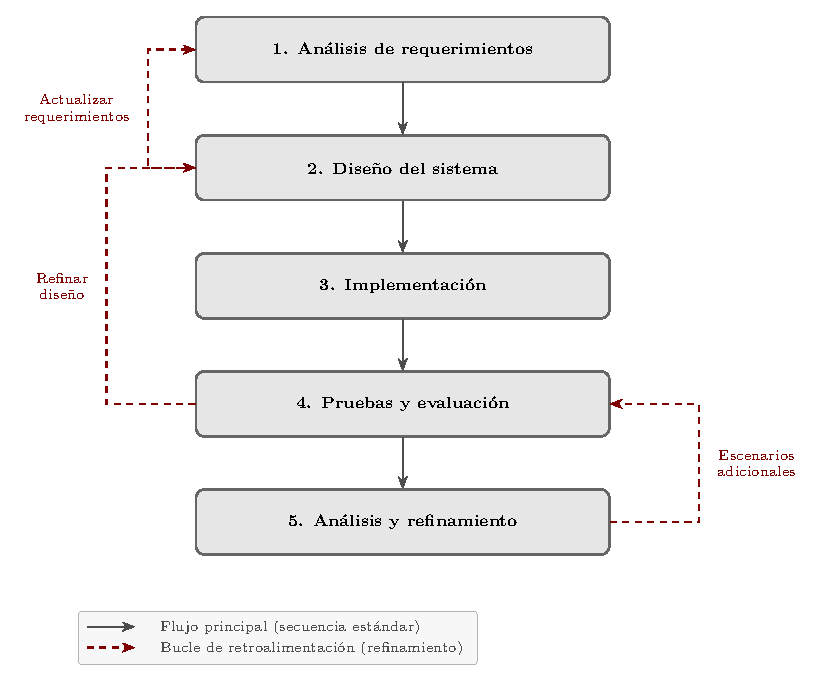
\includegraphics[width=0.80\textwidth]{figures/fig_m1_cascada.pdf}
  \caption{Modelo en cascada retroalimentada adoptado para el desarrollo del proyecto. Las flechas sólidas representan el flujo de trabajo principal; las punteadas, los caminos de retroalimentación que permiten regresar a fases anteriores cuando los resultados lo exigen.}
  \label{fig:cascada}
\end{figure}

El trabajo se organiza en seis fases: (1) \emph{requerimientos y revisión del estado del arte}, donde se definen los requerimientos del estudio y se construye el marco teórico; (2) \emph{análisis del escenario}, donde se caracterizan la geometría del enlace LEO y los parámetros NPRACH; (3) \emph{diseño del sistema}, donde se definen los bloques del modelo y las adaptaciones sobre los principios de SARA y NORA (el resto de este capítulo); (4) \emph{implementación} de los módulos en el simulador ---capa física LEO, canal, detector de colisiones, scheduler NPRACH, codebooks SCMA y decodificador MPA--- documentada en el \cref{ch:implementacion}; (5) \emph{verificación y validación} de cada módulo contra resultados publicados; y (6) \emph{análisis de resultados y conclusiones} (\cref{ch:resultados}), donde se ejecutan las campañas de simulación variando la carga de UEs y se comparan las métricas de los tres esquemas.

Los caminos de realimentación de la \cref{fig:cascada} operan así: si las métricas no cumplen los criterios de aceptación (\cref{sec:design_criterios}), se revisan parámetros del diseño (como el umbral $\Delta d_{\min}$ del agrupamiento o la política de asignación de codebooks); si durante el diseño aparece un requerimiento faltante, se actualiza el listado de requerimientos (\cref{sec:requerimientos}); y el análisis de resultados puede sugerir escenarios adicionales. Esta flexibilidad es la razón principal para escoger la cascada retroalimentada frente a una cascada estrictamente secuencial.

En cuanto a las herramientas, la implementación se realiza en NS-3 (\emph{Network Simulator 3}), un simulador de eventos discretos de código abierto ampliamente usado en la investigación de redes celulares. NS-3 incluye módulos de LTE y NB-IoT, pero su canal radio por defecto está pensado para enlaces terrestres, por lo que requiere las adaptaciones al enlace NTN-LEO descritas en el \cref{ch:implementacion}. El procesamiento posterior de las trazas ---cálculo de métricas, curvas de capacidad y análisis de la matriz de confusión--- se realiza en Python con las bibliotecas pandas, numpy y matplotlib, y el código se gestiona con Git.

\section{Requerimientos del sistema}
\label{sec:requerimientos}
\label{ch:requerimientos}

Esta sección formaliza los requerimientos del procedimiento de acceso aleatorio adaptado para redes no terrestres (NTN) con satélites LEO, expresados de manera independiente de cualquier herramienta de simulación o lenguaje de implementación. Los requerimientos se clasifican en \emph{funcionales}, que describen qué debe hacer el sistema, y \emph{no funcionales}, que describen cómo debe comportarse respecto a rendimiento, compatibilidad y robustez. Se incluyen también las restricciones de diseño impuestas por la capa física NB-IoT y por la normativa 3GPP para NTN.

El trabajo propone dos esquemas de la familia \textbf{CRACS} (\emph{Collision-detected Random Access with Codebook SCMA}): \textbf{CRACS-R} (codebook aleatorio del catálogo) y \textbf{CRACS-T} (codebook por clúster ToA). Ambos comparten el núcleo de detección probabilística de colisión, multiplexación T-SCMA en MSG3 y decodificación MPA, y difieren en la estrategia de asignación de codebook. Por ello, los requerimientos funcionales se clasifican en tres bloques: (i) \emph{compartidos} por ambos esquemas, (ii) específicos de \textbf{CRACS-R}, y (iii) específicos de \textbf{CRACS-T}. La columna \emph{Aplica} de la \cref{tab:rf} explicita esta clasificación.

\subsection{Requerimientos funcionales}
\label{sec:rf}

La \cref{tab:rf} enumera los requerimientos funcionales del sistema. Cada requerimiento se identifica con un código único \texttt{RF-XX} y su cumplimiento se verificará durante la fase de pruebas, ejecutada sobre la implementación documentada en el \cref{ch:implementacion}. Los requerimientos se expresan en términos cualitativos --qué debe hacer el sistema-- sin fijar valores numéricos; las magnitudes concretas (probabilidades del detector, número de codebooks, umbral de agrupamiento, etc.) se establecen como criterios de sistema en los requerimientos no funcionales (\cref{sec:rnf}) y en las restricciones de diseño (\cref{sec:restricciones}), y se concretan más adelante en este capítulo.

\begin{table}[H]
\centering
\caption{Requerimientos funcionales del sistema.}
\label{tab:rf}
\small
\begin{tabularx}{\textwidth}{@{}l X c c@{}}
\toprule
\textbf{ID} & \textbf{Descripción} & \textbf{Aplica} & \textbf{Prioridad} \\
\midrule
RF-01 & El sistema debe modelar la geometría tridimensional del enlace UE--satélite y la dinámica orbital, de modo que cada UE tenga asociados su distancia al satélite, su retardo de propagación y su ángulo de elevación. & Compartido & Alta \\
\addlinespace
RF-02 & El eNB debe detectar de forma probabilística las colisiones de preámbulo en el canal NPRACH. & Compartido & Alta \\
\addlinespace
RF-03 & Cada UE debe transmitir MSG3 sobre la capa SCMA asignada, adjuntando un piloto DMRS tomado del pool anunciado y su identidad de usuario. & Compartido & Alta \\
\addlinespace
RF-04 & El eNB debe decodificar las transmisiones MSG3 superpuestas mediante el decodificador MPA y clasificar cada transmisión --capa propia, capa compartida o colisión de piloto-- para resolver el acceso. & Compartido & Alta \\
\addlinespace
RF-05 & El procedimiento debe resolver de forma concurrente varias entidades (clústeres en CRACS-T o codebooks en CRACS-R) dentro de una misma ventana RACH, hasta el límite que imponga el número de codebooks SCMA disponibles. & Compartido & Media \\
\addlinespace
RF-06 & El procedimiento debe operar bajo el retardo de ida y vuelta extendido del enlace LEO sin alterar las ventanas temporales especificadas para NTN. & Compartido & Alta \\
\addlinespace
RF-07 & Los UEs que no completen el acceso en un intento deben reintentar mediante backoff aleatorio, hasta un número máximo de intentos configurable. & Compartido & Media \\
\addlinespace
RF-08 & Ante una colisión, el eNB debe emitir dos RARs con identificadores temporales distintos, cada uno anunciando el catálogo de codebooks SCMA y el pool de pilotos; cada UE colisionante debe escoger al azar una RAR, un codebook y un piloto antes de transmitir MSG3. & CRACS-R & Alta \\
\addlinespace
RF-09 & El eNB debe agrupar los UEs colisionantes en clústeres disjuntos según su distancia diferencial al satélite. & CRACS-T & Alta \\
\addlinespace
RF-10 & Por cada clúster, el eNB debe emitir una única RAR que provea un identificador temporal compartido, una capa SCMA asignada de forma determinista, la concesión de recurso uplink y la referencia de timing del clúster. & CRACS-T & Alta \\
\bottomrule
\end{tabularx}
\end{table}

\subsection{Requerimientos no funcionales}
\label{sec:rnf}

La \cref{tab:rnf} lista los requerimientos no funcionales. Se expresan como criterios cuantificables verificables contra las métricas de desempeño definidas en la \cref{sec:design_kpis}.

\begin{table}[H]
\centering
\caption{Requerimientos no funcionales del sistema.}
\label{tab:rnf}
\small
\begin{tabularx}{\textwidth}{@{}l X X@{}}
\toprule
\textbf{ID} & \textbf{Descripción} & \textbf{Criterio de aceptación} \\
\midrule
RNF-01 & La complejidad computacional del decodificador MPA debe estar acotada en número de iteraciones por ventana MSG3. & $I_{\text{MPA}} \leq 10$ iteraciones \\
\addlinespace
RNF-02 & El diseño debe ser compatible con la capa física NB-IoT NPUSCH Format~1 y operar sobre una subportadora única de 15 kHz. & Sin modificación al PHY estándar \\
\addlinespace
RNF-03 & El mecanismo de agrupamiento y resolución debe operar sin señalización adicional fuera de la cadena MSG1--MSG5. & Cero mensajes de control extra \\
\addlinespace
RNF-04 & Los parámetros del modelo deben ser trazables a especificaciones 3GPP para NTN. & Correspondencia formal con 3GPP TR~36.763 y TR~38.821 \\
\addlinespace
RNF-05 & CRACS-T debe degradar de forma controlada a comportamiento equivalente a CRACS-R (un único clúster con codebook compartido) cuando $\Delta d_{\min}$ no permite separar a los UEs colisionantes. & Fallback determinista ante proximidad extrema \\
\addlinespace
RNF-06 & El sistema debe ser reproducible: la evaluación debe entregar resultados estadísticamente consistentes. & Media e intervalo de confianza al 95\% con al menos 30 repeticiones \\
\addlinespace
RNF-07 & El detector probabilístico de colisiones debe ofrecer una fiabilidad suficiente para no degradar el acceso por detecciones omitidas o falsas alarmas. & $p_{\text{det}} \geq 0{,}975$ y $p_{\text{fa}} \leq 0{,}001$ \\
\bottomrule
\end{tabularx}
\end{table}

\subsection{Restricciones de diseño}
\label{sec:restricciones}

El diseño se acota por las siguientes restricciones, derivadas de la especificación NB-IoT y de la viabilidad del decodificador MPA:

\begin{itemize}[leftmargin=*, noitemsep]
  \item \textbf{Ancho de banda uplink.} Una sola subportadora de 15~kHz (NB-IoT NTN no permite multitono en uplink en la banda de interés).
  \item \textbf{Longitud de la ventana T-SCMA.} Máximo $N = 4$ subframes por ventana, alineado con la estructura de dos slots de NPUSCH Format~1.
  \item \textbf{Número de codebooks SCMA.} Máximo $K_{\text{CB}} = 6$, con sobreocupación $K_{\text{CB}}/N = 150\%$, límite práctico de separabilidad del receptor MPA.
  \item \textbf{Ángulo de elevación mínimo.} $\alpha_{\min}$ configurable en el rango $10^\circ$--$30^\circ$, con el compromiso entre cobertura angular y pérdida de enlace.
  \item \textbf{Distancia diferencial mínima.} $\Delta d_{\min} = 150$~m, correspondiente a la resolución temporal del NPRACH a 15~kHz de subportadora.
  \item \textbf{Número de pilotos DMRS ortogonales.} 3 por capa SCMA, máximo teórico de cyclic shifts ortogonales compatibles con $N = 4$ recursos.
  \item \textbf{Preámbulos disponibles.} $N_{\text{pream}} = 48$, conforme a la especificación NB-IoT para RACH.
\end{itemize}

Estas restricciones se asumen fijas durante el diseño y solo se revisan si la fase de evaluación demuestra que su violación es necesaria para alcanzar los objetivos del trabajo.

\section{Modelo de sistema NTN--LEO}
\label{sec:modelo_sistema}

El escenario de estudio consiste en un único satélite LEO en órbita circular que actúa como eNB para una población de terminales NB-IoT estacionarios desplegados sobre una huella terrestre rural. La \cref{fig:system_model} es la representación de referencia del sistema y consolida los elementos geométricos, el modelo de cobertura y los supuestos de canal sobre los que se construye el resto del capítulo. En ella, la geometría queda definida por la altitud orbital $h_{\text{sat}}$, el slant range $d_{\text{slant}}$ entre cada UE y el satélite, el ángulo de elevación local $\alpha$ y el ángulo de elevación mínimo $\alpha_{\min}$ que delimita la cobertura; los UEs se distribuyen uniformemente en un disco de radio $R_{\text{cell}}$ centrado en el punto sub-satelital, y los terminales con elevación inferior a $\alpha_{\min}$ se consideran fuera de servicio.

\begin{figure}[H]
  \centering
  
\includegraphics[width=0.95\textwidth]{esquema_general.jpg}
  \caption{Modelo de sistema NB-IoT sobre un único satélite LEO.}
  \label{fig:system_model}
\end{figure}

Los parámetros numéricos del modelo de referencia se listan en la \cref{tab:parametros}.\footnote{El \emph{nadir} es el punto de la superficie terrestre situado directamente bajo el satélite; el RTT mínimo se da cuando el UE coincide con el nadir y el slant range se reduce a la altitud orbital $h_{\text{sat}}$.}

\begin{table}[H]
\centering
\caption{Parámetros del modelo de sistema.}
\label{tab:parametros}
\small
\begin{tabular}{@{}l c l l@{}}
\toprule
\textbf{Parámetro} & \textbf{Símbolo} & \textbf{Valor de referencia} & \textbf{Fuente} \\
\midrule
Altitud orbital & $h_{\text{sat}}$ & 600 km & 3GPP TR 36.763 \\
Velocidad orbital & $v_{\text{sat}}$ & $\sim$7.5 km/s & Mecánica orbital LEO \\
Ángulo de elevación mínimo & $\alpha_{\min}$ & $10^\circ$--$45^\circ$ (default $40^\circ$) & Configurable \\
RTT mínimo (nadir) & $\mathrm{RTT}_{\min}$ & $\sim$4 ms & Cálculo \\
RTT máximo (borde de cobertura) & $\mathrm{RTT}_{\max}$ & $\sim$27 ms & $\alpha_{\min}=10^\circ$ \\
Pérdida atmosférica & $L_{\text{atm}}$ & $0{,}53$ dB (constante) & Modelo de referencia \\
FSPL promedio & $L_{\text{FSPL}}$ & $150$ dB (constante) & Modelo de referencia \\
Margen de enlace & $L_{\text{margin}}$ & $0{,}82$ dB (constante) & Reserva de diseño \\
Ganancia de antena UE & $G_{\text{UE}}$ & isotrópica & Modelo de referencia \\
\bottomrule
\end{tabular}
\end{table}

La potencia recibida por cada UE activo dentro del cono de cobertura se modela como
\begin{equation}
  P_{\text{RX}} = P_{\text{TX}} - L_{\text{atm}} - L_{\text{FSPL}} - L_{\text{margin}}.
  \label{eq:link_budget}
\end{equation}
Las tres pérdidas se toman constantes; los valores concretos empleados en la evaluación se listan en la \cref{tab:impl_flags}. Los UEs cuya elevación sea inferior a $\alpha_{\min}$ se consideran fuera de servicio mediante un criterio binario (dentro o fuera de cobertura).

\paragraph{Aspectos modelados.} El sistema considera la geometría tridimensional del enlace UE--satélite a partir de las coordenadas ECEF, incluyendo la dinámica orbital del satélite a lo largo del tiempo, el RTT por UE calculado como $2 d_{\text{slant}}/c$, el criterio de cobertura por elevación mínima ($\alpha_{\min}$), que clasifica a cada UE como dentro o fuera de servicio, un balance de enlace con pérdidas atmosféricas y de espacio libre constantes y un margen fijo, y la distancia diferencial $\Delta d = d_{\text{slant}} - h_{\text{sat}}$, magnitud geométrica cuyo papel en el agrupamiento se detalla más adelante en la \cref{sec:cracs_t}.

\paragraph{Aspectos no modelados.} Para concentrar el análisis en el procedimiento de acceso, el modelo asume condiciones ideales de canal y no representa: la variación de FSPL con la distancia ($1/r^2$), el desvanecimiento rápido (Rician o Rayleigh), el sombreado log-normal, el desplazamiento Doppler debido al movimiento del satélite, la atenuación por lluvia y el centelleo ionosférico, el patrón de radiación de las antenas (se asume ganancia isotrópica) y la dispersión por multitrayecto. Estos aspectos se asumen bajo condiciones ideales de canal para concentrar el análisis en el desempeño del procedimiento de acceso; declararlos de forma explícita acota el alcance de validez de los resultados de capacidad.

\paragraph{Asunción de propagación en línea de vista.} El modelo asume canal de propagación en línea de vista entre cada UE en cobertura y el satélite, con pérdidas constantes ($L_{\text{atm}}$, $L_{\text{FSPL}}$, $L_{\text{margin}}$) y un criterio de cobertura de tipo todo-o-nada (el UE está dentro o fuera de servicio) según el ángulo de elevación mínimo. Esta abstracción es consistente con el nivel de detalle propio de un análisis de acceso aleatorio a nivel de sistema, donde el foco no es la caracterización fina del enlace sino el desempeño agregado del procedimiento de acceso bajo carga creciente. Los efectos de propagación más realistas identificados en los \emph{Aspectos no modelados} se reservan como extensiones de trabajo futuro.

\section{Visión general de los esquemas evaluados}
\label{sec:vision}

Este trabajo propone dos esquemas que conforman la familia \textbf{CRACS} (\emph{Collision-detected Random Access with Codebook SCMA}): \textbf{CRACS-R} (codebook aleatorio del catálogo) y \textbf{CRACS-T} (codebook por clúster ToA). Ambos comparten un núcleo común sobre la cadena estándar de acceso aleatorio NB-IoT: (i) un \emph{detector probabilístico de colisiones} de preámbulo en el eNB, (ii) una \emph{multiplexación T-SCMA} del payload MSG3 que permite la resolución simultánea de múltiples UEs mediante decodificación MPA, y (iii) la \emph{individualización por IMSI} en MSG4 cuando varios UEs comparten TC-RNTI. La diferencia entre los dos esquemas radica en la \emph{estrategia de asignación de codebook} SCMA tras detectar una colisión.

\textbf{CRACS-R} adapta el principio de SARA (Moon et al., 2021) al contexto NB-IoT NTN incorporando SCMA: tras detectar colisión, el eNB emite dos RARs anunciando el catálogo completo de codebooks; cada UE elige aleatoriamente un codebook y un piloto DMRS. Es un esquema sin información geométrica adicional, dependiente del azar y de la separación posterior por MPA.

\textbf{CRACS-T} extiende el principio NORA (Wang et al., 2020) incorporando un agrupamiento espacial de los UEs colisionantes basado en su distancia diferencial al satélite, y \emph{asignación determinista} del codebook SCMA por clúster: tras detectar colisión, el eNB analiza los tiempos de llegada de los preámbulos superpuestos, los agrupa en clústeres espaciales y emite una RAR por clúster con TC-RNTI compartido y codebook fijo asignado. Aprovecha la geometría LEO para reducir la contienda residual aguas abajo.

La \cref{tab:esquemas} contrasta los tres esquemas considerados en este trabajo: el baseline Legacy y las dos propuestas CRACS-R y CRACS-T.

\begin{table}[H]
\centering
\caption{Comparación de los tres esquemas considerados.}
\label{tab:esquemas}
\small
\begin{tabularx}{\textwidth}{@{}l X X X@{}}
\toprule
\textbf{Aspecto} & \textbf{Legacy (baseline)} & \textbf{CRACS-R (propuesta 1)} & \textbf{CRACS-T (propuesta 2)} \\
\midrule
Detección de colisión MSG1 & No & Probabilística & Probabilística \\
Agrupamiento espacial & No aplica & No aplica & Sí, por $\Delta d$ \\
RARs emitidos por colisión & 1 (no distingue) & 2 (fijo por diseño) & 1 por clúster \\
Asignación de codebook & No aplica & Catálogo anunciado, sorteo por UE & Determinista por clúster \\
Pilotos DMRS & Únicos por UE & Pool anunciado, sorteo por UE & Pool compartido, sorteo por UE \\
Resolución MSG3 & Ninguna (fallo por superposición) & MPA tras sorteo aleatorio & MPA con contexto de clúster \\
Colisión de pilotos & No aplica & Posible (diseño) & Minimizada (por clustering) \\
Individualización de C-RNTI & TC-RNTI único & Por TC-RNTI distinto o IMSI & Por IMSI en RRC \\
\bottomrule
\end{tabularx}
\end{table}

\section{Arquitectura general del proceso de simulación}
\label{sec:arquitectura}

La \cref{fig:system_arch} resume el flujo general del proceso de simulación que articula los tres esquemas: a partir de los parámetros de entrada se configura el sistema y se construye el escenario; el flujo se bifurca según el esquema de acceso seleccionado (Legacy, CRACS-R o CRACS-T), y finaliza en una etapa común de evaluación de la capacidad del canal.

\begin{figure}[H]
  \centering
  
\includegraphics[width=0.95\textwidth]{fig_m3_system_arch.pdf}
  \caption{Diagrama general del proceso de simulación común a los tres esquemas.}
  \label{fig:system_arch}
\end{figure}

En detalle, cada etapa del diagrama comprende lo siguiente. La etapa de \emph{parámetros de entrada} fija el esquema de acceso bajo prueba (Legacy, CRACS-R o CRACS-T), la semilla de simulación, el perfil de tráfico, la geometría orbital LEO ($h_{\text{sat}}$, $\alpha_{\min}$ y posición central), el modelo de canal y los parámetros del detector probabilístico de colisión (en CRACS-R y CRACS-T). La etapa \emph{configurar el simulador} activa el esquema seleccionado y establece los parámetros del canal LEO y de la temporización NTN. La etapa \emph{construir el escenario} instancia el satélite y los UEs, los distribuye sobre el área de cobertura y genera los tiempos de intento de acceso. Tras ejecutar el esquema seleccionado en la bifurcación, la etapa común \emph{evaluar la capacidad del canal} recopila las métricas registradas durante la simulación y calcula los indicadores de capacidad definidos en la \cref{sec:design_kpis}.

\section{Procedimiento baseline: Legacy}
\label{sec:legacy}

El procedimiento Legacy implementa el acceso aleatorio NB-IoT estándar en cinco mensajes, cada uno con un propósito definido dentro del establecimiento de la conexión: en MSG1 el UE transmite un preámbulo aleatorio (uno entre $N_{\text{pream}} = 48$) para anunciar su intención de acceso y permitir que el eNB estime su retardo de propagación; con MSG2 (RAR) el eNB acusa el preámbulo y entrega los recursos iniciales ---TC-RNTI, \textit{timing advance} y concesión uplink--- que el UE necesita para transmitir de forma sincronizada; en MSG3 (RRC Connection Request) el UE se identifica y solicita formalmente el establecimiento de la conexión; con MSG4 (RRC Connection Setup) el eNB resuelve la contienda y asigna el identificador definitivo (C-RNTI); y MSG5 (RRC Setup Complete) cierra el procedimiento confirmando que la conexión quedó establecida. La \cref{fig:legacy} ilustra el flujo de éxito (a) y el escenario de colisión (b).

\begin{figure}[H]
  \centering
  
\includegraphics[width=0.95\textwidth]{fig2_legacy_msc.pdf}
  \caption{Procedimiento de acceso aleatorio baseline (Legacy): flujo de éxito y escenario de colisión.}
  \label{fig:legacy}
\end{figure}

En la \cref{fig:legacy} las etiquetas se presentan en forma genérica: solo se identifican los mensajes intercambiados (MSG1--MSG5 con sus campos: RAPID, TC-RNTI, TA, UL Grant, C-RNTI) y la tarea ejecutada a cada lado (selección de preámbulo en el UE; detección, asignación de TC-RNTI, construcción de la RAR y decodificación de MSG3 en el eNB). El tamaño del pool de preámbulos disponibles ($N_{\text{pream}} = 48$) y el resto de parámetros numéricos se enuncian en el párrafo previo.

En el escenario de colisión, el eNB observa un único pico de correlación NPRACH para el RAPID colisionado y emite una sola RAR con un único TC-RNTI. Los UEs colisionantes reciben idéntica RAR y responden con MSG3 sobre el mismo recurso PUSCH. La superposición de las transmisiones impide la decodificación: el eNB no recibe ningún MSG3 válido y la ventana de contienda expira. Los UEs retransmiten el preámbulo tras un backoff aleatorio.

\section{Primera propuesta: CRACS-R (codebook aleatorio del catálogo)}
\label{sec:cracs_r}

\textbf{CRACS-R} es la primera propuesta de la familia CRACS. Adapta el principio de SARA (Moon et al., 2021) al contexto NB-IoT NTN incorporando SCMA en MSG3 y detección probabilística de colisión en el eNB. Es un esquema deliberadamente \emph{sin información geométrica}: la separación de UEs colisionantes se delega íntegramente al sorteo aleatorio de codebooks y pilotos seguido de decodificación MPA. La \cref{fig:sara} ilustra el flujo con tres UEs colisionantes.

\begin{figure}[H]
  \centering
  
\includegraphics[width=0.95\textwidth]{fig3_sara_msc.pdf}
  \caption{Procedimiento CRACS-R con tres UEs colisionantes.}
  \label{fig:sara}
\end{figure}

En la \cref{fig:sara} las etiquetas se presentan en forma genérica (sin valores ni índices específicos): solo se identifican los mensajes y las tareas. Las probabilidades del detector ($p_{\text{det}}=0{,}975$, $p_{\text{fa}}=0{,}001$), el tamaño del catálogo de codebooks SCMA ($K_{\text{CB}}=6$), la cardinalidad del pool de pilotos DMRS ($D=3$) y la cantidad fija de RARs emitidos por colisión (\emph{dos}) se enuncian en los ítems del listado que sigue.

Los puntos clave del diseño de CRACS-R son:
\begin{itemize}[leftmargin=*, noitemsep]
  \item \textbf{Detección probabilística}: el eNB dispone de un detector con probabilidad $p_{\text{det}} = 0.975$ y $p_{\text{fa}} = 0.001$; sin embargo, solo conoce \emph{que} ocurrió una colisión, no cuántos UEs están involucrados.
  \item \textbf{Dos RARs fijos}: dado que el mínimo para que exista colisión es de dos UEs, el eNB emite siempre dos RARs, cada uno con un TC-RNTI distinto y con el catálogo completo de capas SCMA ($K = 6$) y de pilotos DMRS ($D = 3$).
  \item \textbf{Elección aleatoria del UE}: cada UE selecciona una RAR al azar (lo que implica que dos UEs pueden terminar compartiendo TC-RNTI) y, en MSG3, una capa SCMA y un piloto DMRS al azar del pool anunciado.
  \item \textbf{Resolución por MPA}: el eNB decodifica las transmisiones MSG3 superpuestas mediante MPA. Si dos UEs eligieron la misma capa y el mismo piloto (colisión de piloto), ambos fallan; en otros casos, el eNB puede separarlos.
  \item \textbf{Individualización en RRC}: cuando los UEs comparten TC-RNTI, la individualización del C-RNTI se realiza en MSG4 usando el IMSI transmitido en el RRC Connection Request.
\end{itemize}

\section{Segunda propuesta: CRACS-T (codebook por clúster ToA)}
\label{sec:cracs_t}

\textbf{CRACS-T} es la segunda propuesta de la familia CRACS. Extiende el principio NB-NORA introducido por Wang \emph{et al.} (2020) incorporando agrupamiento espacial de los UEs colisionantes basado en su distancia diferencial al satélite y \emph{asignación determinista} del codebook SCMA por clúster. Aprovecha la dispersión de tiempos de llegada característica del enlace LEO para particionar los UEs colisionantes \emph{antes} de emitir las RARs, reduciendo la contienda residual aguas abajo. La \cref{fig:new} ilustra el flujo completo con tres UEs que caen en un mismo clúster.

\begin{figure}[H]
  \centering
  
\includegraphics[width=0.95\textwidth]{fig4_new_msc.pdf}
  \caption{Procedimiento de acceso aleatorio de CRACS-T con tres UEs colisionantes agrupados en un mismo clúster.}
  \label{fig:new}
\end{figure}

En la \cref{fig:new} las etiquetas se presentan en forma genérica: solo se identifican los mensajes intercambiados, los pasos del procedimiento y las tareas ejecutadas a cada lado (detección probabilística + agrupamiento por ToA en el eNB; verificación de pertenencia al clúster en el UE; decodificación MPA e individualización por IMSI). Las probabilidades del detector ($p_{\text{det}}=0{,}975$, $p_{\text{fa}}=0{,}001$), el umbral de separación $\Delta d_{\min}=150$~m, el tamaño del catálogo de codebooks ($K_{\text{CB}}=6$) y el pool de pilotos DMRS ($D=3$) se detallan en los pasos del flujo descritos a continuación.

El flujo se descompone en los cinco pasos siguientes:

\subsection*{Paso 1: Transmisión de preámbulo y registro de timing}
Cada UE selecciona un preámbulo al azar y lo transmite en MSG1. En el instante de transmisión, el UE registra su \emph{timing advance} actual, calculado como la distancia diferencial $\Delta d = d_{\text{slant}} - h_{\text{sat}}$. Este valor se almacena localmente y se usará en el paso 2 para confirmar la pertenencia al clúster anunciado por el eNB. El eNB, al recibir MSG1, ejecuta el detector probabilístico de colisiones.

\subsection*{Paso 2: Agrupamiento y emisión de RAR de clúster}
Si se detecta colisión en un RAPID, el eNB ordena los tiempos de llegada de los preámbulos superpuestos y realiza un barrido de clustering: dos preámbulos pertenecen al mismo clúster si su separación en $\Delta d$ es inferior a $\Delta d_{\min}$. El número de clústeres resultantes está acotado por $K_{\text{CB}}$. Por cada clúster, el eNB emite una única RAR que contiene (i) un TC-RNTI compartido, (ii) una capa SCMA determinista asignada al clúster, (iii) la concesión uplink, y (iv) el valor de $\Delta d$ representativo del clúster.

Al recibir la RAR, cada UE compara el valor $\Delta d$ recibido con el que registró al transmitir MSG1. Si la diferencia es menor que $\Delta d_{\min}/2$, el UE adopta la RAR como propia.

\subsection*{Paso 3: Transmisión MSG3 multiplexada}
Todos los UEs del mismo clúster transmiten MSG3 sobre la misma capa SCMA asignada, usando un piloto DMRS seleccionado aleatoriamente del pool ortogonal (3 pilotos disponibles). El payload incluye el IMSI del UE (necesario para la individualización en RRC). Las transmisiones se superponen sobre los $N = 4$ subframes de la ventana T-SCMA.

\subsection*{Paso 4: Resolución MPA y emisión de MSG4}
El eNB recibe la señal superpuesta y ejecuta el algoritmo MPA sobre el grafo de factores $\mathbf{F}_{4\times 6}$ (cuya estructura y propósito ---separar las transmisiones SCMA superpuestas explotando la esparsidad del codebook--- se detallan en la \cref{sec:scma}). Por cada UE cuya transmisión sea decodificable, el eNB extrae el IMSI del payload y asigna un C-RNTI individual. MSG4 se envía sobre el TC-RNTI compartido pero contiene el IMSI y el C-RNTI específicos por UE, permitiendo que cada UE identifique su propia respuesta.

\subsection*{Paso 5: Confirmación}
Cada UE decodifica MSG4, identifica su IMSI en el payload, adopta el C-RNTI asignado y confirma con MSG5 (RRC Setup Complete). Los UEs que no recibieron respuesta (por colisión de piloto o fallo de MPA) entran en backoff y reintentan desde el paso 1.

\section{Mecanismo de agrupamiento por tiempo de llegada (CRACS-T)}
\label{sec:toa}

El agrupamiento por tiempo de llegada es el rasgo distintivo de \textbf{CRACS-T} respecto a CRACS-R: es lo que le permite asignar codebooks SCMA de forma determinista en lugar de aleatoria. La \cref{fig:toa} ilustra cómo se particionan los UEs colisionantes en clústeres disjuntos según su distancia diferencial al satélite.

\begin{figure}[H]
  \centering
  
\includegraphics[width=0.95\textwidth]{fig5_toa_clustering.pdf}
  \caption{Mecanismo de agrupamiento por distancia diferencial $\Delta d$. Los UEs colisionantes se ordenan por su $\Delta d$ y se agrupan en clústeres separados por al menos $\Delta d_{\min} = 150$~m. Cada clúster recibe una RAR con TC-RNTI compartido y una capa SCMA asignada de forma determinista.}
  \label{fig:toa}
\end{figure}

Las decisiones de diseño clave son:
\begin{description}[leftmargin=1.5em,style=nextline]
  \item[Por qué $\Delta d$ y no $d_{\text{slant}}$:] la resta $d_{\text{slant}} - h_{\text{sat}}$ elimina el sesgo común dado por la altitud orbital, dejando la métrica invariante respecto a la posición instantánea del satélite. Esto hace el agrupamiento robusto frente a la deriva orbital entre MSG1 y MSG2.
  \item[Por qué $\Delta d_{\min} = 150$~m:] este valor corresponde a la resolución temporal efectiva del NPRACH con subportadora de 15~kHz. UEs más cercanos que este umbral no son separables por timing y deben tratarse como un único clúster (fallback a comportamiento CRACS-R dentro del clúster).
  \item[Algoritmo de agrupamiento:] se ordenan los valores $\Delta d$ observados en orden ascendente y se realiza un barrido lineal que abre un nuevo clúster cada vez que la separación con el anterior supera $\Delta d_{\min}$. La complejidad es $O(K \log K)$ en el número $K$ de UEs colisionantes.
  \item[Salida:] una partición $\{C_1, C_2, \ldots, C_M\}$ de los UEs colisionantes en $M$ clústeres disjuntos, con $M \leq K_{\text{CB}} = 6$.
\end{description}

\section{SCMA y grafo de factores}
\label{sec:scma}

La multiplexación SCMA empleada en MSG3 se apoya en un grafo de factores bipartito $\mathbf{F}_{N \times K}$ con $N = 4$ recursos (subframes) y $K = 6$ codebooks. La \cref{fig:factor_graph} presenta la estructura del grafo y la matriz indicadora que lo codifica.

\begin{figure}[H]
  \centering
  
\includegraphics[width=0.85\textwidth]{fig6_factor_graph.pdf}
  \caption{Grafo de factores SCMA $\mathbf{F}_{4 \times 6}$. Los nodos de función (rectángulos) representan los cuatro elementos de recurso; los nodos de variable (círculos) representan los seis codebooks. Cada codebook ocupa $d_v = 2$ recursos y cada recurso acomoda $d_f = 3$ codebooks, con una sobreocupación $K/N = 150\%$.}
  \label{fig:factor_graph}
\end{figure}

Las propiedades del grafo relevantes al diseño son: el grado de cada nodo de función $d_f = 3$ determina cuántos codebooks se superponen en un mismo recurso; el grado de cada nodo de variable $d_v = 2$ determina cuántos recursos utiliza cada codebook (esparsidad temporal); el número total de codebooks es $K = \binom{N}{d_v} = \binom{4}{2} = 6$, lo que agota el espacio combinatorio y garantiza que cada codebook ocupe un patrón distinto.

\section{Diseño T-SCMA para el uplink MSG3}
\label{sec:tscma}

La multiplexación SCMA se implementa en el dominio del tiempo siguiendo la técnica T-SCMA propuesta por Yan \emph{et al.} (2017) específicamente para NB-IoT, ya que el ancho de banda de una subportadora de 15~kHz no admite multiplexación clásica en frecuencia. Apoyándose en el grafo de factores de la \cref{fig:factor_graph}, la \cref{fig:tscma_multiplex} ilustra cómo se organiza la transmisión paralela de $K = 6$ codebooks sobre $N = 4$ subframes en una única subportadora de 15~kHz, mientras que la \cref{fig:tscma_symbol} detalla la estructura de símbolo dentro de un subframe activo.

\begin{figure}[H]
  \centering
  
\includegraphics[width=0.95\textwidth]{fig8_tscma_design.pdf}
  \caption{Patrón de multiplexación T-SCMA. La cuadrícula muestra los seis UEs (filas) y los cuatro subframes (columnas). Cada celda activa indica que el UE transmite en ese subframe (datos más piloto DMRS); las celdas \emph{silent} indican subframes en los que el UE no transmite. En cada subframe se acumulan hasta $d_f = 3$ codebooks que se superponen en el aire y producen una única forma de onda compuesta por subframe en el receptor.}
  \label{fig:tscma_multiplex}
\end{figure}

\begin{figure}[H]
  \centering
  
\includegraphics[width=0.92\textwidth]{fig9_tscma_symbol.pdf}
  \caption{Estructura de símbolo dentro de un subframe activo (NPUSCH Format~1, 15~kHz). El subframe se compone de catorce símbolos OFDM organizados en dos slots de siete. Los pilotos DMRS ocupan los símbolos 3 y 10; los doce símbolos restantes transportan datos. La estructura es idéntica para cada celda activa de la \cref{fig:tscma_multiplex}; aquí se ilustra con el color del UE$_1$/CB$_1$ a modo de ejemplo.}
  \label{fig:tscma_symbol}
\end{figure}

Las decisiones de diseño para T-SCMA son:
\begin{description}[leftmargin=1.5em,style=nextline]
  \item[Dominio del tiempo en lugar de frecuencia:] NB-IoT opera con una única subportadora uplink de 15~kHz, lo que imposibilita la multiplexación en frecuencia clásica. El tiempo (subframes) es el único eje disperso disponible.
  \item[Cuatro subframes:] se alinea con la estructura estándar de NPUSCH Format~1 (2 slots de 7 símbolos cada uno). Permite mantener la compatibilidad con la especificación PHY sin modificaciones.
  \item[Piloto DMRS por UE:] cada UE transmite su DMRS en los símbolos 3 y 10 de los subframes en los que su codebook está activo. Las secuencias DMRS son ortogonales entre sí (hasta un máximo de 3 por capa), lo que permite al receptor distinguir las contribuciones individuales superpuestas.
  \item[Superposición en el aire:] las señales de los UEs activos en un mismo subframe se suman coherentemente en el canal. El eNB recibe una única forma de onda compuesta por subframe.
\end{description}

\paragraph{Procedimiento T-SCMA en cinco pasos.} \textbf{(i)}~Cada UE recibe un codebook entre los $K = 6$ disponibles. \textbf{(ii)}~El UE mapea sus datos a una palabra-código de longitud $N = 4$ con solo $d_v = 2$ posiciones no nulas (esparsidad temporal). \textbf{(iii)}~En cada uno de sus dos subframes asignados, el UE transmite símbolos de datos en las posiciones de datos e inserta su propio piloto DMRS en los símbolos 3 y 10 (\cref{fig:tscma_symbol}). \textbf{(iv)}~Hasta $d_f = 3$ UEs transmiten en paralelo en un mismo subframe; los datos se superponen en el aire y los pilotos DMRS, con secuencias Zadoff--Chu distintas, permanecen separables. \textbf{(v)}~El eNB captura una única forma de onda compuesta por subframe, correlaciona contra las secuencias DMRS conocidas para detectar UEs activos y estimar canales, y aplica MPA iterativo para separar los datos superpuestos.

\section{Lógica de resolución MSG3 en el eNB}
\label{sec:resolucion}

La decodificación MSG3 en el eNB sigue una lógica de tres niveles que clasifica cada transmisión recibida como \emph{scheduled}, \emph{contender con colisión de piloto}, o \emph{contender decodificable por MPA}. La \cref{fig:decision} presenta el árbol de decisión formal.

\begin{figure}[H]
  \centering
  
\includegraphics[width=0.90\textwidth]{fig7_decision_tree.pdf}
  \caption{Árbol de decisión del procedimiento de resolución MSG3 en el eNB. Cada transmisión recibida se clasifica en uno de los cuatro casos posibles según si el UE es único en su capa SCMA, si sufre colisión de piloto, o si su señal es decodificable por MPA con probabilidad $p_{\text{BD}}(d_c)$.}
  \label{fig:decision}
\end{figure}

La lógica procede así. Tras cerrarse la ventana de recepción de MSG3, el eNB identifica, para cada capa SCMA, cuántos UEs la están ocupando y qué pilotos DMRS han utilizado. Luego, para cada transmisión recibida:
\begin{enumerate}[leftmargin=*]
  \item \textbf{¿El UE es único ocupante de su capa SCMA?} Si es así, el UE se declara \emph{scheduled}: el eNB conoce totalmente el contexto de su transmisión y la decodifica con probabilidad $p_{\text{BD}} = 1$, sin invocar MPA.
  \item \textbf{¿Otro UE seleccionó la misma pareja (capa, piloto)?} Si es así, ocurre \emph{colisión de piloto}: ambos UEs son indistinguibles para el receptor y ambos fallan. Deberán reintentar el acceso.
  \item \textbf{¿El receptor MPA decodifica la señal?} En otro caso, el eNB invoca MPA sobre el grafo de factores; la probabilidad de decodificación $p_{\text{BD}}(d_c)$ depende del nivel de superposición $d_c$ de la capa. Un resultado exitoso produce el payload del UE y permite la asignación de C-RNTI; un fallo genera un reintento.
\end{enumerate}

La \cref{tab:msg3_casos} resume los cuatro casos posibles y la acción correspondiente del eNB.

\begin{table}[H]
\centering
\caption{Casos de resolución MSG3 en el eNB.}
\label{tab:msg3_casos}
\small
\begin{tabularx}{\textwidth}{@{}l c X X X@{}}
\toprule
\textbf{Caso} & \textbf{Aplica a} & \textbf{Condición} & \textbf{Acción del eNB} & \textbf{Resultado del UE} \\
\midrule
Éxito directo & CRACS-T & UE único en su capa SCMA asignada (clúster con un solo UE) & Aceptar sin invocar MPA & C-RNTI asignado \\
Éxito por MPA & ambas & Pilotos DMRS distintos en la misma capa & MPA converge con $\mathrm{LLR} \geq$ umbral & C-RNTI asignado \\
Colisión de piloto & ambas & Dos o más UEs con misma pareja (capa, piloto) & Descarte de todos los involucrados & Retransmisión tras backoff \\
Fallo de decodificación & ambas & MPA no converge o densidad $d_c$ excesiva & NACK implícito (no emite MSG4) & Retransmisión tras backoff \\
\bottomrule
\end{tabularx}
\end{table}

El caso \emph{Éxito directo} (UE único en su capa SCMA) solo aplica a \textbf{CRACS-T}: la asignación determinista de codebook por clúster permite que algunos UEs sean los únicos ocupantes de su capa, evitando la invocación de MPA. En \textbf{CRACS-R} todos los UEs comparten el catálogo de codebooks vía sorteo aleatorio, por lo que cualquier UE colisionante siempre necesita resolución por MPA (o falla por colisión de piloto).

La probabilidad $p_{\text{BD}}(d_c)$ se modela como una función decreciente del número de UEs activos simultáneamente en la capa (densidad de colisión $d_c$). La \cref{tab:pbd_calib} resume los valores de referencia adoptados, calibrados empíricamente sobre la base de la literatura SCMA y de las corridas iniciales de la fase de evaluación.

\begin{table}[H]
\centering
\caption{Probabilidad de decodificación blind $p_{\text{BD}}(d_c)$ del receptor MPA.}
\label{tab:pbd_calib}
\small
\renewcommand{\arraystretch}{1.15}
\begin{tabular}{@{}c c l@{}}
\toprule
$d_c$ & $p_{\text{BD}}$ & Régimen operativo \\
\midrule
$\leq 2$ & $1{,}00$ & Por debajo de la carga nominal \\
$3$      & $0{,}95$ & Carga nominal, cerca de ML \\
$4$      & $0{,}85$ & Un contendor añadido \\
$5$      & $0{,}70$ & Dos contendores añadidos \\
$\geq 6$ & $\leq 0{,}05$ & Sobrecarga severa \\
\bottomrule
\end{tabular}
\end{table}

En la \cref{fig:decision} solo aparecen los nombres de los nodos de decisión y las acciones resultantes; las probabilidades específicas se consultan en la \cref{tab:pbd_calib}.

\section{Indicadores de desempeño del diseño}
\label{sec:design_kpis}

La evaluación del diseño se apoya en un conjunto de indicadores clave de desempeño (KPIs) que cuantifican la calidad del procedimiento de acceso desde tres perspectivas complementarias: \emph{éxito} (cuántos UEs completan el acceso), \emph{latencia} (cuánto tarda el acceso exitoso) y \emph{eficiencia} (qué costo tiene en reintentos y colisiones). Adicionalmente, CRACS-T expone un indicador propio de calidad del agrupamiento espacial. La \cref{tab:design_kpis} formaliza las definiciones; estos KPIs son los que se reportan en el capítulo de resultados (\cref{ch:resultados}).

\begin{table}[H]
\centering
\caption{Indicadores clave de desempeño (KPIs) del procedimiento de acceso.}
\label{tab:design_kpis}
\small
\begin{tabularx}{\textwidth}{@{}l c X l@{}}
\toprule
\textbf{KPI} & \textbf{Símbolo} & \textbf{Definición} & \textbf{Unidad} \\
\midrule
Tasa de acceso exitoso & SAR & Fracción de UEs que completan MSG1--MSG5 dentro de $\mathrm{PT}_{\max}$ intentos & $[0, 1]$ \\
\addlinespace
SAR de primer intento & $\text{SAR}_{1}$ & Fracción de UEs que completan el acceso en el primer envío de MSG1 & $[0, 1]$ \\
\addlinespace
Latencia de acceso & $T_{\text{access}}$ & Tiempo entre MSG1 y MSG4 sobre UEs exitosos. Se reporta media, mediana ($p50$) y percentil 95 ($p95$) & ms \\
\addlinespace
Latencia del intento exitoso & $T_{\text{inst}}$ & Tiempo entre el último MSG1 (el que tuvo éxito) y MSG4. La diferencia $T_{\text{access}} - T_{\text{inst}}$ cuantifica el costo de los reintentos & ms \\
\addlinespace
Probabilidad de éxito antes de $T$ (SDP) & $\mathrm{SDP}(T)$ & Fracción del \emph{total} de UEs (incluidos fallidos) que completaron el acceso en tiempo $\leq T$. Métrica conjunta latencia--confiabilidad ($T \in \{1, 3, 10\}$\,s) & $[0, 1]$ \\
\addlinespace
Tiempo total de servicio & TST & \emph{Makespan} de la oleada: $\max(t_{\text{MSG4}}) - \min(t_{\text{MSG1}})$ sobre UEs exitosos & ms \\
\addlinespace
ECDF del retardo de acceso & --- & Distribución empírica acumulada del retardo de acceso por esquema, normalizada por el total de UEs (satura en el SAR) & --- \\
\addlinespace
Tasa de colisión de preámbulo & $\mathrm{PCR}_{\text{pre}}$ & Fracción de transmisiones MSG1 que comparten preámbulo con otra transmisión simultánea & $[0, 1]$ \\
\addlinespace
Tasa de colisión de piloto MSG3 & $\mathrm{PCR}_{\text{msg3}}$ & Fracción de transmisiones MSG3 que comparten la misma pareja (capa SCMA, piloto DMRS) con otra en la misma ventana & $[0, 1]$ \\
\addlinespace
Throughput de acceso & $\eta_{\text{ra}}$ & Accesos exitosos por segundo & UE/s \\
\addlinespace
Reintentos & $\text{RTX}_{\text{mean}}$, $\text{RTX}_{\text{max}}$ & Promedio y peor caso de envíos de MSG1 por UE antes del éxito o agotamiento & --- \\
\addlinespace
Identificación correcta de clúster & CID & Fracción de UEs cuyo clúster asignado por el eNB coincide con la partición geométrica de referencia. Solo aplica a CRACS-T & $[0, 1]$ \\
\bottomrule
\end{tabularx}
\end{table}

\section{Regiones operativas esperadas (hipótesis ex-ante)}
\label{sec:design_regiones}

Como hipótesis \emph{ex-ante} del diseño, los tres esquemas cubren regiones operativas de tamaño progresivamente mayor en el plano \emph{(carga $K$, RTT del enlace)}. La \cref{fig:regiones} visualiza esta hipótesis: el esquema Legacy opera con éxito únicamente en cargas bajas y RTT cortos; CRACS-R amplía el rango de carga aceptable mediante la multiplexación SCMA de MSG3; y CRACS-T extendería además la tolerancia al RTT al desacoplar la separación temporal del MSG3 mediante el agrupamiento espacial previo, sustituyendo el sorteo aleatorio de codebook por una asignación determinista por clúster.

\begin{figure}[H]
  \centering
  
\includegraphics[width=0.95\textwidth]{fig_m2_param_map.pdf}
  \caption{Regiones operativas esperadas de los tres esquemas en función de la carga $K$ y el RTT del enlace. Se conjetura la inclusión estricta Legacy $\subset$ CRACS-R $\subset$ CRACS-T, hipótesis ex-ante que será contrastada experimentalmente en el \cref{ch:resultados}.}
  \label{fig:regiones}
\end{figure}

Formalmente, denotando $\Omega_X \subset \mathbb{R}^2$ la región de parámetros $(K, \mathrm{RTT})$ donde el esquema $X$ mantiene $\mathrm{SAR} \geq \mathrm{SAR}_{\text{umbral}}$, se conjetura la inclusión
\begin{equation}
  \Omega_{\text{Legacy}} \subsetneq \Omega_{\text{CRACS-R}} \subsetneq \Omega_{\text{CRACS-T}},
  \label{eq:inclusion}
\end{equation}
con inclusiones estrictas. Esta conjetura define el horizonte de éxito del diseño propuesto. \emph{Su validez se contrasta empíricamente en el \cref{ch:resultados}, donde los datos revelan que la inclusión es condicional al timer T300 --- un hallazgo no anticipado por el diseño que refina el espacio operativo de la familia CRACS.}

\section{Criterios de aceptación del diseño}
\label{sec:design_criterios}

Los esquemas propuestos se consideran satisfactorios si los resultados experimentales cumplen los siguientes criterios cuantitativos \emph{ex-ante} sobre los KPIs definidos en la \cref{sec:design_kpis}:

\begin{enumerate}[leftmargin=*]
  \item \textbf{Mejora en tasa de acceso:} $\mathrm{SAR}_{\text{CRACS-T}} > \mathrm{SAR}_{\text{CRACS-R}}$ para toda carga $K \geq 3$, con intervalo de confianza al $95\%$.
  \item \textbf{Costo de latencia aceptable:} $T_{\text{access, CRACS-T}} \leq 1{,}1 \cdot T_{\text{access, CRACS-R}}$ en los mismos escenarios; CRACS-T no debe introducir un aumento de latencia superior al $10\%$ respecto a CRACS-R.
  \item \textbf{Precisión del agrupamiento (CRACS-T):} $\mathrm{CID} \geq 0{,}95$ para $\Delta d_{\min} = 150$~m bajo distribución espacial uniforme. Una degradación bajo este umbral exige revisar el parámetro de agrupamiento.
  \item \textbf{Reducción de colisión de piloto:} $\mathrm{PCR}_{\text{msg3, CRACS-T}} \leq 0{,}5 \cdot \mathrm{PCR}_{\text{msg3, CRACS-R}}$ para toda carga $K$. Esta reducción refleja el efecto del agrupamiento determinista sobre la contienda residual en MSG3.
  \item \textbf{Escalabilidad:} ambas propuestas deben mantener $\mathrm{SAR} \geq 0{,}8$ para $K \leq K_{\text{CB}} = 6$ (régimen operativo nominal) y degradar de forma progresiva para cargas superiores.
\end{enumerate}

El no cumplimiento de cualquiera de estos criterios indica una limitación del diseño en el rango operativo correspondiente y debe documentarse explícitamente en la fase de análisis. \emph{La validez condicional de estos criterios --- en particular C1 y C2, que dependen del timer T300 según se muestra en el \cref{ch:resultados} --- se discute en detalle en el capítulo de resultados.}

\section{Plan de evaluación}
\label{sec:metodologia}

Esta sección operacionaliza la fase de pruebas del modelo en cascada descrito en la \cref{sec:metodologia_desarrollo}: define cómo se evalúa el diseño con independencia del entorno de implementación. Se especifican las variables del experimento, los escenarios de evaluación y las condiciones de borde. Las métricas de desempeño son los KPIs ya definidos en la \cref{sec:design_kpis} y los criterios de aceptación contra los que se contrastan los resultados son los enunciados en la \cref{sec:design_criterios}; ninguno se repite aquí.

\subsection{Diseño experimental}
\label{sec:dis_simulacion}

La fase de evaluación se operacionaliza, con independencia del entorno de implementación, manipulando un conjunto de variables sobre el sistema diseñado. Las \textbf{variables independientes} son: la carga $K$ (número de UEs activos en la ventana de acceso); el modelo de tráfico (Poisson uniforme, 3GPP TR~37.868 TM1, o Beta$(3,4)$ sincronizado, TM2); el perfil de tráfico (\emph{avg} moderado o \emph{high} intenso, $\lambda \approx 27{,}8$~UEs/s); la distancia diferencial mínima de agrupamiento $\Delta d_{\min}$ (propia de CRACS-T); el número de preámbulos NPRACH $N_{\text{pream}}$; el temporizador RRC $T_{300}$ (valores estándar NB-IoT, 3GPP TS~36.331); y el esquema bajo prueba (Legacy, CRACS-R o CRACS-T). Los demás parámetros geométricos del enlace ($h_{\text{sat}}$, $\alpha_{\min}$, FSPL constante) se fijan en los valores de referencia documentados en la \cref{sec:modelo_sistema}, ya que el alcance del trabajo es la capacidad del canal de acceso bajo una geometría LEO de referencia y no la sensibilidad a las variables de canal. Las \textbf{variables dependientes} son los KPIs definidos en la \cref{sec:design_kpis} (\cref{tab:design_kpis}).

\textbf{Modelos estadísticos y condiciones de ejecución.} Cada UE inicia su acceso en un instante aleatorio dentro de la ventana $T_{\text{arrival}}$, según la distribución uniforme (caso base) o Beta$(3,4)$ (caso mMTC, 3GPP TR~37.868); los UEs se ubican uniformemente en el disco de cobertura definido por $\alpha_{\min}$ ---distribución espacial neutra, que no privilegia ninguna zona de la huella y representa un despliegue IoT rural sin agrupamiento geográfico previo--- y permanecen estáticos durante cada ejecución independiente del simulador, denominada en adelante \emph{corrida}. Los que fallan un intento reintentan con backoff uniforme hasta un máximo de $\mathrm{PT}_{\max}=10$ intentos, tras lo cual se consideran perdidos. Cada punto experimental se repite con al menos $R=30$ semillas independientes y se reporta como media con intervalo de confianza al 95\% (método $t$ de Student); el tiempo simulado de referencia es $T_{\text{sim}}=120$~s por experimento, suficiente para que todos los UEs completen el procedimiento o agoten sus reintentos. Por corrida se registran los eventos de la cadena MSG1--MSG5 con sus metadatos (UE ID, RAPID, TC-RNTI, capa SCMA, piloto DMRS), que el post-procesamiento agrega por escenario y esquema para calcular los KPIs.

\subsection{Escenarios de evaluación}
\label{sec:escenarios}

Cada escenario aísla una variable independiente y barre su rango manteniendo las demás en los valores de referencia; las variantes \emph{\_high} repiten el barrido bajo el perfil de tráfico intenso ($\lambda \approx 27{,}8$~UEs/s), que satura el canal de acceso. La \cref{tab:escenarios} los resume; la operacionalización exacta de cada uno sobre el simulador se detalla en el \cref{ch:implementacion}.

\begin{table}[H]
\centering
\caption{Escenarios de evaluación.}
\label{tab:escenarios}
\small
\begin{tabularx}{\textwidth}{@{}l l l l X@{}}
\toprule
\textbf{ID} & \textbf{Variable} & \textbf{Rango} & \textbf{Esquemas} & \textbf{Propósito} \\
\midrule
E0 & $K$ & 1 UE & los 3 & \emph{Sanity}: equivalencia de los tres esquemas sin contienda \\
\addlinespace
E1 & $K$ (perfil avg) & 1--100 UEs & los 3 & Curva de capacidad bajo tráfico moderado \\
\addlinespace
E1\_high & $K$ (perfil high $2\text{h}$) & 1--100 UEs & los 3 & Curva de capacidad bajo tráfico intenso \\
\addlinespace
E4 & $\Delta d_{\min}$ (perfil avg) & 50--1000 m & CRACS-T & Calibración del parámetro de agrupamiento \\
\addlinespace
E4\_high & $\Delta d_{\min}$ (perfil high) & 50--1000 m & CRACS-T & Idem bajo tráfico intenso \\
\addlinespace
E5 & $N_{\text{pream}}$ (perfil avg) & 12, 24, 36, 48 & los 3 & Sensibilidad al pool de preámbulos NPRACH \\
\addlinespace
E5\_high & $N_{\text{pream}}$ (perfil high) & 12, 24, 36, 48 & los 3 & Idem bajo tráfico intenso \\
\addlinespace
E6\_uniform & $K$ (Poisson TM1, $T=60$\,s) & 30, 100, 300, 1000 & los 3 & Saturación con tráfico no correlacionado \\
\addlinespace
E6\_burst & $K$ (Beta$(3,4)$ TM2, $T=10$\,s) & 30, 100, 300, 1000 & los 3 & Saturación con ráfaga sincronizada \\
\addlinespace
E7\_t300 & $T_{300}$ (en E6\_burst $K{=}300$) & 5, 10, 40 s & los 3 & Sensibilidad al timer T300 en el punto de cruce \\
\bottomrule
\end{tabularx}
\end{table}

\subsection{Condiciones de borde}
\label{sec:borde}

La evaluación incluye un conjunto de casos límite de control: con $K=1$ los tres esquemas deben comportarse idénticamente, pues no hay colisión posible (cualquier divergencia indicaría un defecto de modelado); para $K > K_{\text{CB}} = 6$ ambas propuestas deben degradar de forma controlada, lo que delimita el rango operativo máximo; cuando todos los UEs caen en un único clúster ($\Delta d < \Delta d_{\min}$), el comportamiento de CRACS-T converge al de CRACS-R; y con $p_{\text{fa}} > 0$ se observa el impacto de las falsas alarmas del detector probabilístico sobre la asignación de RARs.
